\documentclass[10pt]{beamer}
\usetheme{Madrid}
\usecolortheme{whale}

% --- PACKAGES ---
\usepackage[utf8]{inputenc}
\usepackage[T1]{fontenc}
\usepackage[french]{babel}
\usepackage{multirow}
\usepackage{xcolor}
\usepackage{graphicx}
\usepackage{multicol}
\usepackage{booktabs}
\usepackage{microtype}
\usepackage{listings}
\usepackage{fontawesome5}
\usepackage{appendixnumberbeamer}
\usepackage{hyperref}
\usepackage{array}
\usepackage{amssymb}
\usepackage{amsmath}
\usepackage{caption}
\usepackage{tikz}
\usetikzlibrary{mindmap,trees,shapes.geometric,arrows.meta,decorations.pathreplacing,calc,shadows, shadows.blur,positioning,patterns,backgrounds}
\usepackage{pgfplots}
\pgfplotsset{compat=1.18}
\usepackage{tcolorbox}
\tcbuselibrary{skins,breakable}

% --- COULEURS ---
\definecolor{donecolor}{RGB}{46,125,50}
\definecolor{todoColor}{RGB}{251,140,0}
\definecolor{undonecolor}{RGB}{198,40,40}
\definecolor{team1color}{RGB}{33,150,243}
\definecolor{team2color}{RGB}{233,30,99}
\definecolor{team3color}{RGB}{255,152,0}
\definecolor{team4color}{RGB}{0,150,136}
\definecolor{umlcolor}{RGB}{0,102,204}
\definecolor{codebg}{RGB}{245,248,250}
\definecolor{accentcolor}{RGB}{156,39,176}
\definecolor{graycircle}{RGB}{200,200,200}
\definecolor{cardbg}{RGB}{250,250,252}
\definecolor{softblue}{RGB}{227,242,253}
\definecolor{softgreen}{RGB}{232,245,233}
\definecolor{softorange}{RGB}{255,243,224}
\definecolor{softpurple}{RGB}{243,229,245}

% Style listings
\lstset{
    basicstyle=\ttfamily\small,
    backgroundcolor=\color{codebg},
    frame=single,
    rulecolor=\color{gray!30},
    tabsize=2,
    showstringspaces=false
}


% tcolorbox style corrigé
\tcbset{
    modern/.style={
        enhanced,
        arc=5pt,
        boxrule=1.2pt,
        drop shadow,
        fontupper=\small
    }
}

% Configuration Beamer modernisée
\setbeamertemplate{footline}[frame number]
\setbeamercolor{page number in head/foot}{fg=black}
\setbeamertemplate{navigation symbols}{}
\setbeamertemplate{section in toc}[sections numbered]
\setbeamertemplate{subsection in toc}[subsections numbered]
\setbeamertemplate{caption}[numbered]
\setbeamertemplate{headline}{}
\graphicspath{{./images/}}


\setbeamertemplate{background}{
    \begin{tikzpicture}[overlay, remember picture]
        \fill[team1color!50] (current page.south east) rectangle ++(-1.5,0.8);
        \fill[team1color!30] (current page.south west) rectangle ++(0.5,0.8);
        \fill[team1color!10] (current page.north west) rectangle (current page.south east);
    \end{tikzpicture}
}

% Style blocs modernisés
\setbeamercolor{block title}{bg=team1color, fg=white}
\setbeamercolor{block body}{bg=softblue}
\setbeamercolor{alertblock title}{bg=undonecolor, fg=white}
\setbeamercolor{alertblock body}{bg=softorange}


\title{{\large \texttt{Projet de conception logicielle 3 -- Jeu de Tron}}}
\author{
    \textit{Équipe de développement :}\\[0.2cm]
    {\small
    \begin{tabular}{|c|l|c|}
        \hline
        \textbf{N°} & \textbf{Prénom et nom} & \textbf{Numéro} \\ \hline
        1 & Lamia \textbf{HADJ BENABDELMOULA} & 22409436 \\ \hline
        2 & Selssabil \textbf{KHELALFA} & 22403233 \\ \hline
        3 & Oumar \textbf{BAH} & 22409261 \\ \hline
        4 & Thierno Hammady \textbf{DIALLO} & 22409301 \\ \hline
    \end{tabular}}
    \\[0.2cm]
    \textbf{Chargé de TP :} M. Alexis \textsc{Lechervy}
}
\date{\small \textit{Présenté le \today}}

\begin{document}

% ==================== SLIDE 1 : TITRE ====================
\begin{frame}
    \begin{center}
        
\includegraphics[width=0.25\linewidth]{images/logos.png} \\
        \vspace{-0.1cm}
        \texttt{\large Licence 3 Informatique}
    \end{center}
    \vspace{-0.3cm}
    \titlepage
\end{frame}

% ==================== SLIDE 2 : PLAN ====================
\begin{frame}{Plan de la présentation}
    \centering
    \begin{minipage}{0.8\textwidth}
        \small
        \tableofcontents[hideallsubsections]
    \end{minipage}
\end{frame}

% ==================== SLIDE 3 : CONTEXTE ====================
\section{Contexte du projet}
\begin{frame}{Présentation du projet}
    \begin{columns}[T]
        \begin{column}{0.6\textwidth}
            \vspace{0.2cm}
            \begin{itemize}
                \item Tron est une variante multi-joueurs du jeu du serpent.
                \item Les joueurs se déplacent sur une grille et laissent derrière eux une trace qui devient un obstacle.
                \item Tous les déplacements modifient l'espace disponible pour les autres joueurs.
                \item Le but est de survivre plus longtemps que les autres, seul ou en équipe.
                \item Ce cadre est intéressant pour étudier des comportements multi-agents et des décisions automatiques.
            \end{itemize}
        \end{column}
        \begin{column}{0.35\textwidth}
            \centering
            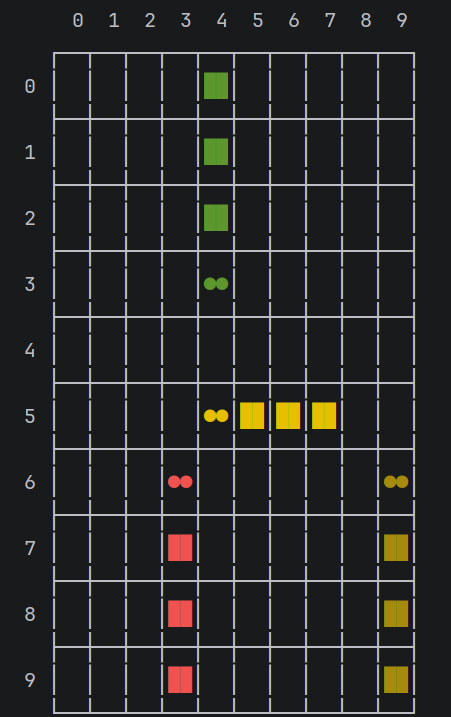
\includegraphics[width=\linewidth]{images/jeu.png}
        \end{column}
    \end{columns}
\end{frame}

% ==================== SLIDE 4 : PROBLEMATIQUE ====================
\section{Problématique et objectifs du projet}
\begin{frame}{Problématique et objectifs}
    \begin{block}{Problématique}
        Comment comparer des stratégies de décision dans un jeu de Tron multi-joueurs, en tenant compte des équipes, des heuristiques et de la profondeur de recherche ?
    \end{block}

    \begin{tcolorbox}[enhanced, arc=5pt, colback=softgreen, colframe=donecolor, title=Objectifs du projet]
        \begin{itemize}
            \item Construire un jeu de Tron multi-joueurs jouable automatiquement.
            \item Mettre en place plusieurs stratégies d'intelligence artificielle.
            \item Ajouter des heuristiques pour évaluer les positions.
            \item Lancer des expérimentations pour comparer les comportements obtenus.
        \end{itemize}
    \end{tcolorbox}
\end{frame}

% ==================== SLIDE 5 : ARCHITECTURE ====================
\section{Architecture et modélisation}

\begin{frame}{Idée générale de l'architecture}
    \begin{tcolorbox}[enhanced, arc=5pt, colback=softblue, colframe=team1color, title=Concept clé]
        Le projet a été construit pour séparer clairement la logique du jeu, l'affichage et le contrôle de la partie. Cela permet de modifier une partie du système sans devoir tout réécrire.
    \end{tcolorbox}

    \vspace{0.5cm}
    \centering
    \begin{tikzpicture}[node distance=0.7cm, >=stealth, thick, scale=0.8, transform shape]
        % Modèle principal
        \node[fill=team1color!15, , text width=0.45\textwidth,
        align=center, draw=team1color, thick, minimum height=1.2cm, drop shadow] (mod)
        {\faCube\ \textbf{Modèle indépendant}};

        % Observer
        \node[fill=team2color!15, , text width=0.32\textwidth,
        align=center, draw=team2color, thick, minimum height=1cm,
        above left=0.8cm and -1.5cm of mod, drop shadow] (obs)
        {\small \faEye\ \textbf{Pattern Observer}};

        % Strategy
        \node[fill=team3color!15, , text width=0.32\textwidth,
        align=center, draw=team3color, thick, minimum height=1cm,
        above right=1.2cm and -1.5cm of mod, drop shadow] (strat)
        {\small \faChess\ \textbf{Pattern Strategy}};

        % Extension
        \node[fill=donecolor!15, , text width=0.45\textwidth,
        align=center, draw=donecolor, thick, minimum height=1.2cm,
        below=0.8cm of mod, drop shadow] (ext)
        {\faExpand\ \textbf{Ajout facile de nouvelles IA et heuristiques}};

        % Flèches
        \draw[->, team1color, line width=1.5pt] (obs.south) -- (mod.north west);
        \draw[->, team1color, line width=1.5pt] (strat.south) -- (mod.north east);
        \draw[->, donecolor, line width=1.5pt] (mod.south) -- (ext.north);
    \end{tikzpicture}
\end{frame}

\begin{frame}{Architecture MVC}
    \centering
    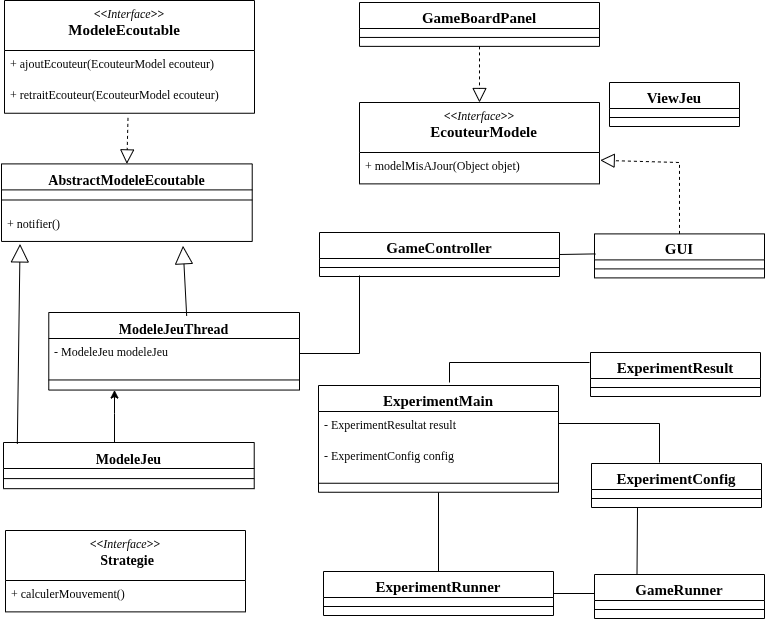
\includegraphics[width=0.86\linewidth]{images/dia.png}
\end{frame}

% ==================== SLIDE 6 : RÉPARTITION ====================
\section{Répartition des tâches réalisées}
\begin{frame}{Répartition des tâches}
\centering
\renewcommand{\arraystretch}{1.3}
\begin{tabular}{|m{3cm}|m{8.2cm}|}
    \hline
    
    \textbf{Développeur(se)} & \textbf{Implémentations réalisées} \\
    \hline
    \textbf{Oumar} &
    \begin{itemize}
        \item Modèle et cœur du jeu
        \item Mise en place de l'architecture MVC
        \item Participation à l'interface graphique
    \end{itemize} \\
    \hline
    \textbf{Lamia} &
    \begin{itemize}
        \item Pattern Strategy
        \item Classes de test
        \item UML et script d'expérimentation
    \end{itemize} \\
    \hline
    \textbf{Selssabil} &
    \begin{itemize}
        \item Interface graphique
        \item Contrôleur et orchestration du jeu
        \item Diagrammes d'analyse
    \end{itemize} \\
    \hline
    \textbf{Hammady} &
    \begin{itemize}
        \item Modèle et logique de jeu
        \item Heuristiques et évaluateurs
        \item Analyse et expérimentation des stratégies
    \end{itemize} \\
    \hline
\end{tabular}
\end{frame}

% ==================== SLIDE 7 : TECHNOLOGIES ====================
\section{Technologies et outils utilisés}
\begin{frame}{Technologies et outils utilisés}
    \centering
    \resizebox{0.9\textwidth}{!}{%
    \begin{tikzpicture}[
        title/.style={font=\bfseries\color{white}, align=center, minimum height=0.6cm, text width=3.2cm},
        card/.style={rectangle, draw=gray!20, thick, fill=cardbg, rounded corners=10pt, text width=3.2cm, minimum height=3.2cm, align=center, inner sep=5pt, drop shadow},
        node distance=1cm and 0.8cm
    ]
        \node[title, fill=team1color] (tit1) {Développement};
        \node[card, below=0pt of tit1] (card1) {
            \vspace{0.2cm} {\Huge \faJava} \\ \textbf{Java 17} \\
            \vspace{0.3cm} \hrule \vspace{0.2cm}
            {\large \faWindowMaximize} \\ \textbf{Swing}
        };

        \node[title, fill=donecolor, right=of tit1] (tit2) {Conception \& doc};
        \node[card, below=0pt of tit2] (card2) {
            \vspace{0.2cm} {\Huge \faProjectDiagram} \\ \textbf{UML 2.5} \\
            \vspace{0.3cm} \hrule \vspace{0.2cm}
            {\large \faPencilRuler} \\ \textbf{Draw.io}
        };

        \node[title, fill=undonecolor, right=of tit2] (tit3) {Versionnement};
        \node[card, below=0pt of tit3] (card3) {
            \vspace{0.2cm} {\Huge \faGit*} \\ \textbf{Git} \\
            \vspace{0.3cm} \hrule \vspace{0.2cm}
            {\large \faGithub} \\ \textbf{GitHub}
        };

        \node[title, fill=team3color, below=4.2cm of tit1] (tit4) {Build \& scripts};
        \node[card, below=0pt of tit4] (card4) {
            \vspace{0.2cm} {\Huge \faCogs} \\ \textbf{Apache Ant} \\
            \vspace{0.3cm} \hrule \vspace{0.2cm}
            {\large \faTerminal} \\ \textbf{Bash / Shell}
        };

        \node[title, fill=accentcolor, right=of tit4] (tit5) {Analyse \& tests};
        \node[card, below=0pt of tit5] (card5) {
            \vspace{0.2cm} {\Huge \faChartPie} \\ \textbf{JFreeChart} \\
            \vspace{0.3cm} \hrule \vspace{0.2cm}
            {\large \faFlask} \\ \textbf{JUnit 4}
        };

        \node[title, fill=black!60, right=of tit5] (tit6) {Rédaction};
        \node[card, below=0pt of tit6] (card6) {
            \vspace{0.2cm} {\Huge \faFileCode} \\ \textbf{\LaTeX} \\
            \vspace{0.3cm} \hrule \vspace{0.2cm}
            {\large \faChalkboardTeacher} \\ \textbf{Beamer}
        };
    \end{tikzpicture}}
\end{frame}

% ==================== SLIDE 8 : DÉMONSTRATION ====================
\section{Démonstration du jeu}

\begin{frame}{Exemple d'exécution d'une partie avec l'interface graphique}
    \begin{figure}
        \centering
        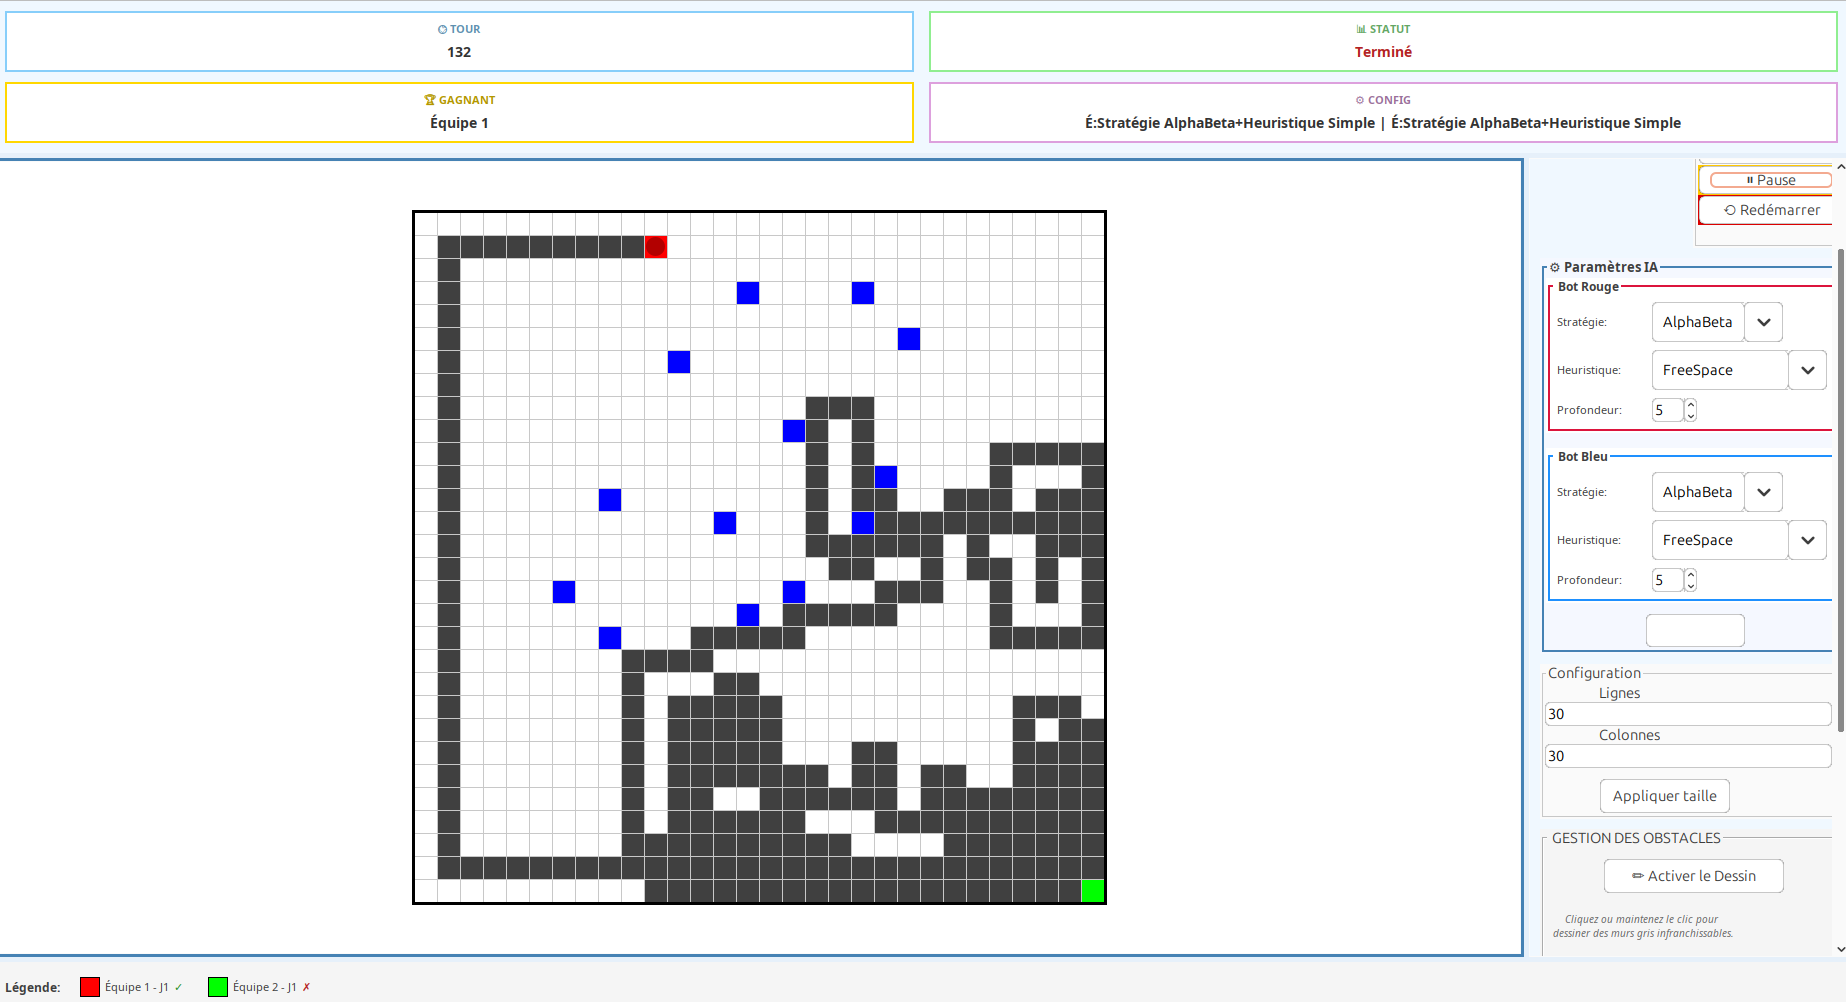
\includegraphics[width=1\linewidth]{images/im7.png}
        \caption{Exemple d'exécution d'une partie avec l'interface graphique}
    \end{figure}
\end{frame}

   
\begin{frame}{Exemple d'exécution d'une partie avec l'interface console}
    \begin{figure}
        \centering
        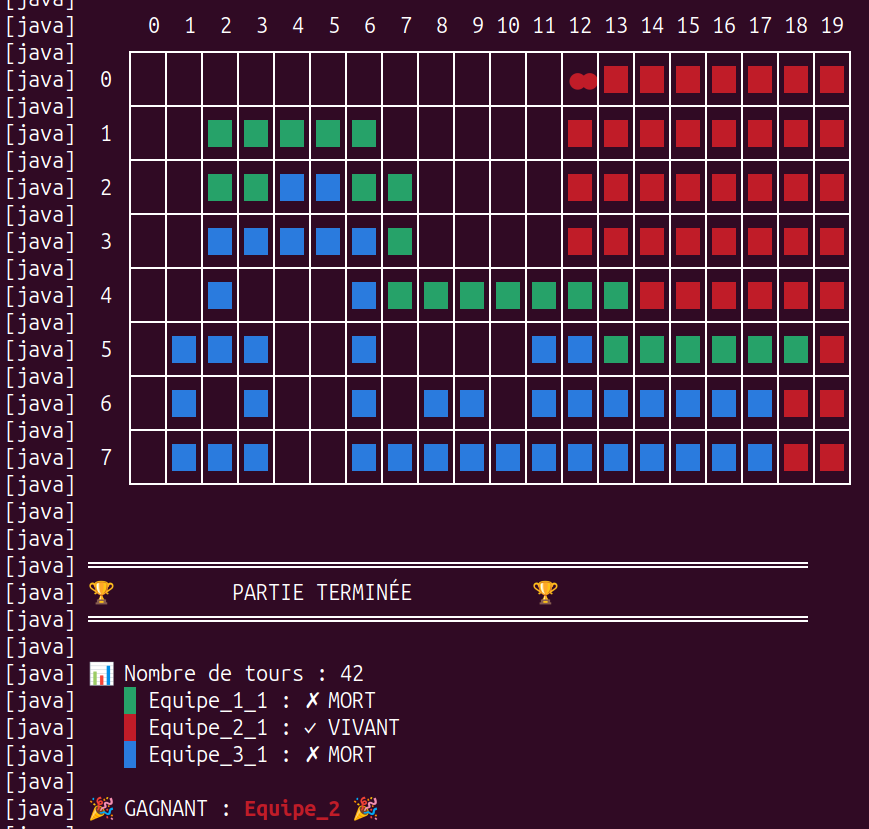
\includegraphics[width=0.7\linewidth]{images/console.png}
        \caption{Exemple d'exécution d'une partie avec l'interface console}
    \end{figure}
\end{frame}

% ==================== SLIDE 9 : STRATÉGIES ====================
\section{Stratégies d'intelligence artificielle}

\begin{frame}{Les 5 stratégies implémentées}
    \centering
    \begin{tikzpicture}[
        node distance=0.8cm,
        algo/.style={rectangle, rounded corners=6pt, draw=team1color!70, thick, fill=team1color!10, minimum width=3cm, minimum height=1cm, align=center, font=\small, drop shadow},
        arrow/.style={->, thick, team1color!50}
    ]
        \node[font=\bfseries\Large, text=team1color] at (0,3) {Algorithmes de recherche};
        
        \node[algo, fill=team2color!10, draw=team2color!70] (minmax) at (-3,1.5) {MinMax};
        \node[algo, fill=team2color!10, draw=team2color!70] (alphabeta) at (3,1.5) {Alpha-Beta};
        \node[font=\small\bfseries, team2color!80] at (0,2.2) {\textbf{Pour 2 joueurs}};
        
        \node[algo, fill=donecolor!10, draw=donecolor!70] (maxn) at (-3.5,-0.5) {MaxN};
        \node[algo, fill=todoColor!10, draw=todoColor!70] (paranoid) at (0,-0.5) {Paranoid};
        \node[algo, fill=accentcolor!10, draw=accentcolor!70] (sos) at (3.5,-0.5) {SOS};
        \node[font=\small\bfseries, donecolor!80] at (0,0.2) {\textbf{Pour N joueurs}};
        
        
        \node[font=\tiny, align=center] at (0,-2) {
            $\bullet$ MinMax/Alpha-Beta : compétition à 2\\[0.1cm]
            $\bullet$ MaxN/Paranoid/SOS : extension à N joueurs
        };
    \end{tikzpicture}
\end{frame}


% ==================== SLIDE 11 : MINMAX ====================
\begin{frame}{MinMax - Schéma de l'arbre}
    \centering
    \begin{tikzpicture}[
        level distance=1.8cm,
        level 1/.style={sibling distance=4cm},
        level 2/.style={sibling distance=1cm},
        maxnode/.style={circle, draw=team2color!70, thick, fill=team2color!20, minimum size=0.6cm, font=\bfseries},
        minnode/.style={circle, draw=team1color!70, thick, fill=team1color!20, minimum size=0.6cm, font=\bfseries},
        leaf/.style={circle, draw=gray!50, thick, fill=gray!20, minimum size=0.5cm, font=\small}
    ]
        \node[maxnode] (root) {MAX}
            child { node[minnode] (min1) {MIN}
                child { node[leaf] (l1) {10} }
                child { node[leaf] (l2) {5} }
                child { node[leaf] (l3) {8} }
            }
            child { node[minnode] (min2) {MIN}
                child { node[leaf] (l4) {3} }
                child { node[leaf] (l5) {12} }
                child { node[leaf] (l6) {7} }
            }
            child { node[minnode] (min3) {MIN}
                child { node[leaf] (l7) {9} }
                child { node[leaf] (l8) {4} }
                child { node[leaf] (l9) {6} }
            };
        
        \node[team1color!80, font=\bfseries] at (root.north) [yshift=0.3cm] {MAX choisit 5};
        
        \draw[->, thick, donecolor!70] (root) -- (min1);
    \end{tikzpicture}
    
\end{frame}

% ==================== SLIDE 12 : ALPHA-BETA ====================
\begin{frame}{Alpha-Beta - Principe de l'élagage}
    \centering
    \begin{tikzpicture}[
        level distance=1.2cm,
        level 1/.style={sibling distance=3.5cm},
        level 2/.style={sibling distance=1.8cm},
        maxnode/.style={circle, draw=team2color!70, thick, fill=team2color!20, minimum size=0.6cm},
        minnode/.style={circle, draw=team1color!70, thick, fill=team1color!20, minimum size=0.6cm},
        leaf/.style={circle, draw=gray!50, thick, fill=gray!20, minimum size=0.5cm}
    ]
        \node[maxnode] (root) {MAX}
            child { node[minnode] (min1) {MIN}
                child { node[leaf] (l1) {5} }
                child { node[leaf] (l2) {3} }
                child[draw=none] { node[draw=none] (empty1) {} edge from parent[draw=none] }
            }
            child { node[minnode] (min2) {MIN}
                child { node[leaf] (l3) {8} }
                child[draw=none] { node[draw=none] (empty2) {} edge from parent[draw=none] }
                child[draw=none] { node[draw=none] (empty3) {} edge from parent[draw=none] }
            };
        
        \draw[undonecolor!80, thick, dashed] (min2.east) -- ++(1.5,0) node[right, undonecolor!80] {\textbf{Branche élaguée}};
        \draw[undonecolor!80, thick, dashed] (min1.east) -- ++(1.2,0);
        
        \node[font=\small, team1color!80] at (root.north) [yshift=0.3cm] {$\alpha = -\infty, \beta = +\infty$};
        \node[font=\small, team1color!80] at (min1.south) [yshift=-1.8cm] {$\alpha = 5, \beta = 3 \rightarrow$ élagage};
    \end{tikzpicture}
    
    \vspace{0.3cm}
    \begin{enumerate}
        \item \textbf{Avantages :} Même résultat que \textit{MinMax} mais beaucoup plus rapide
        \item \textbf{Inconvénient :} Nécessite un bon ordre des coups. Si on explore les mauvaises trajectoires en premier, l'algorithme ne pourra pas couper de branches.
    \end{enumerate}
\end{frame}

% ==================== SLIDE 13 : MAXN VECTEUR ====================
\begin{frame}{MaxN - Le vecteur de scores}
    \centering
    \begin{tikzpicture}
        \draw[thick, fill=team1color!10] (0,0) rectangle (8,1);
        \draw[thick] (2.67,0) -- (2.67,1);
        \draw[thick] (5.33,0) -- (5.33,1);
        
        \node[font=\bfseries, team2color] at (1.33,0.5) {Score Rouge};
        \node[font=\bfseries, team1color] at (4,0.5) {Score Bleu};
        \node[font=\bfseries, donecolor] at (6.67,0.5) {Score Vert};
        
        \node[font=\large] at (1.33,-0.5) {42};
        \node[font=\large] at (4,-0.5) {15};
        \node[font=\large] at (6.67,-0.5) {38};
        
        \draw[->, thick, team2color] (1.33,-0.8) -- (1.33,-1.4)
            node[below, team2color, align=center] {Rouge\\ maximise};

        \draw[->, thick, team1color] (4,-0.8) -- (4,-1.4)
            node[below, team1color, align=center] {Bleu\\ maximise};

        \draw[->, thick, donecolor] (6.67,-0.8) -- (6.67,-1.4)
            node[below, donecolor, align=center] {Vert\\ maximise};
        
        \node[font=\bfseries, text=team1color] at (4,1.5) {Vecteur d'utilité : $[s_R, s_B, s_V]$};
    \end{tikzpicture}
    
    \vspace{0.5cm}
    \begin{tcolorbox}[enhanced, arc=5pt, colback=softgreen, colframe=donecolor, title=Principe MaxN]
        \centering
        Chaque joueur maximise \textbf{sa propre case} dans le vecteur
    \end{tcolorbox}
\end{frame}

% ==================== SLIDE 14 : PARANOID VS MAXN ====================
\begin{frame}{MaxN vs Paranoid : deux logiques antagonistes}
\vspace{1pt}
    \begin{columns}[T]
        \begin{column}{0.50\textwidth}
            \begin{tcolorbox}[colback=green!5, colframe=donecolor, title=\faUsers\ MaxN, rounded corners]
                \centering
                \vspace{0.1cm}
                {\Huge \faChartLine}\\[0.1cm]
                \textbf{\textcolor{donecolor}{Principe :}} Chacun maximise \textbf{son propre score}\\[0.1cm]
                \begin{itemize}
                    \item Vision \textbf{individualiste}
                    \item Chaque joueur agit pour lui-même
                    \item Comportement : \textcolor{donecolor}{\textit{Égoïste}}
                \end{itemize}
                \vspace{0.5cm}
                \small\faQuoteLeft~~ Je veux être le meilleur ! ~~\faQuoteRight
            \end{tcolorbox}
        \end{column}
        
        \begin{column}{0.50\textwidth}
            \begin{tcolorbox}[colback=orange!5, colframe=todoColor, title=\faShield*\ Paranoid, rounded corners]
                \centering
                \vspace{0.1cm}
                {\Huge \faFrown}\\[0.1cm]
                \textbf{\textcolor{todoColor}{Principe :}} Tous les adversaires minimisent \textbf{MON score}\\[0.2cm]
                \begin{itemize}
                    \item Vision \textbf{pessimiste}
                    \item Tous les adversaires sont en coalition
                    \item Comportement : \textcolor{todoColor}{\textit{Défensif}}
                \end{itemize}
                \vspace{0.3cm}
                \small\faQuoteLeft~~ Ils sont tous contre moi ! ~~\faQuoteRight
            \end{tcolorbox}
        \end{column}
    \end{columns}
\end{frame}

% ==================== SLIDE 15 : SOS ====================
\begin{frame}{SOS - Stratégie coopérative}
    \centering
    \begin{tikzpicture}
        \draw[thick, fill=accentcolor!10] (0,0) rectangle (6,1);
        \draw[thick] (2,0) -- (2,1);
        \draw[thick] (4,0) -- (4,1);
        
        \node[font=\bfseries] at (1,0.5) {$s_{\text{Rouge}}$};
        \node[font=\bfseries] at (3,0.5) {$s_{\text{Bleu}}$};
        \node[font=\bfseries] at (5,0.5) {$s_{\text{Vert}}$};
        
        \node[font=\large, accentcolor] at (1,-0.5) {15};
        \node[font=\large, accentcolor] at (3,-0.5) {15};
        \node[font=\large, accentcolor] at (5,-0.5) {15};
        
        \draw[->, thick, accentcolor] (1,-0.8) -- (1,-1.2);
        \draw[->, thick, accentcolor] (3,-0.8) -- (3,-1.2);
        \draw[->, thick, accentcolor] (5,-0.8) -- (5,-1.2);
        
        \node[font=\bfseries, text=accentcolor] at (3,1.5) {SOS = utilité sociale identique};
        \node[font=\small] at (3,2) {Tous les joueurs reçoivent la même valeur !};
    \end{tikzpicture}
    
    \vspace{0.5cm}
    \begin{tcolorbox}[enhanced, arc=5pt, colback=softpurple, colframe=accentcolor, title=Principe SOS]
        \centering
        Maximise le \textbf{bien collectif}, pas l'intérêt individuel.
    \end{tcolorbox}
\end{frame}

% ==================== SLIDE 18 : HEURISTIQUES ====================
\begin{frame}{Les 3 heuristiques implémentées}
    \centering
    \renewcommand{\arraystretch}{1.5}
    \begin{tabular}{|l|c|c|}
        \hline
        
        \textbf{Heuristique} & \textbf{Principe} & \textbf{Coût} \\
        \hline
        
        FreeSpace & Espace de manœuvre restant & Faible \\
        
        Voronoi & Territoire contrôlé & Moyen \\
        
        TreeOfChambers & Structure des espaces libres & Élevé \\
        \hline
    \end{tabular}
    
    \vspace{0.5cm}
    \begin{tikzpicture}
        \draw[thick, fill=donecolor!30] (0,0) rectangle (1.5,0.5);
        \draw[thick, fill=team2color!30] (1.8,0) rectangle (3.3,0.5);
        \draw[thick, fill=accentcolor!30] (3.6,0) rectangle (5.1,0.5);
        
        \node at (0.75,0.25) {Simple};
        \node at (2.55,0.25) {Moyen};
        \node at (4.35,0.25) {Complexe};
        
        \draw[->, thick, team1color] (1.6,0.25) -- (1.7,0.25);
        \draw[->, thick, team1color] (3.4,0.25) -- (3.5,0.25);
        
        \node[fontupper=\tiny] at (2.55,-0.4) {Précision croissante $\rightarrow$};
    \end{tikzpicture}
    
    \vspace{0.5cm}
    \begin{tcolorbox}[enhanced, arc=5pt, colback=softorange, colframe=todoColor, title=Impact sur les algorithmes]
        \centering
        \textbf{Une bonne heuristique peut changer complètement le classement des stratégies !}
    \end{tcolorbox}
\end{frame}
% ==================== SLIDE 19 : PROTOCOLE ====================
\section{Analyse et expérimentation}
\begin{frame}{Protocole expérimental retenu}
    \begin{center}
        \begin{tikzpicture}
            % Ligne 1
            \node[draw=none] (l1) at (0,1.5) {
                \begin{tabular}{cccc}
                    \faUsers & \faTh & \faSearch & \faGamepad \\
                    \textbf{Duel} & \textbf{10/15/20} & \textbf{3/6/9 } & \textbf{50 parties} \\
                    2 équipes & taille & profondeur & par config
                \end{tabular}
            };
            
            % Flèche
            \draw[->, thick, team1color!50] (0,0.5) -- (0,-0.2);
            
            
        \end{tikzpicture}
    \end{center}
    
    \vspace{0.3cm}
    
    \begin{tcolorbox}[colback=softorange!10, colframe=todoColor, rounded corners, font=\small]
        \centering
        \faExclamationTriangle~~\textbf{ Des positions aléatoires }\\   \faExclamationTriangle~~\textbf{protocole en duel pour plus de lisibilité}
    \end{tcolorbox}
\end{frame}

% ==================== SLIDE 20 : MULTITHREADING ====================
\begin{frame}{Multithreading et automatisation}
    \begin{columns}[T]
        \begin{column}{0.70\textwidth}
            \begin{itemize}
                \item \textbf{Pool de threads} dans le mode expérimentation
                \item Plusieurs parties en \textbf{parallèle}
                \item \textbf{MaxN} : parallélisme à la racine
                \item Temps de calcul \textbf{réduit}
            \end{itemize}
        \end{column}
        
        \begin{column}{0.35\textwidth}
            \centering
            \begin{tikzpicture}[>=stealth, thick]
                % Le Noeud Central (Pool)
                \node[circle, draw=team1color, thick, fill=softblue, inner sep=15pt, drop shadow] (pool) at (0,0) {\Large \faMicrochip};
                \node[below=6pt, font=\bfseries] at (pool.south) {Pool de threads};
                
                % Les flèches sortant du haut du cercle vers les tâches
                \draw[->, donecolor] (pool.north east) -- (1.2, 1.2) node[above, text=black] {Partie 1};
                \draw[->, donecolor] (pool.north)      -- (0, 1.5)   node[above, text=black] {Partie 2};
                \draw[->, donecolor] (pool.north west) -- (-1.2, 1.2) node[above, font=\tiny, text=black] {Partie N};
                
                \node[draw=donecolor!50, dashed, rounded corners, fill=white, below=20pt] at (pool.south) {Calculs simultanés};
            \end{tikzpicture}
        \end{column}
    \end{columns}
    \vspace{0.3cm}
    \begin{tcolorbox}[colback=softgreen!10, colframe=donecolor, rounded corners]
        \centering
        \Large \faRocket~~ \textbf{plusieurs configurations}\\
        \normalsize en quelques heures !
    \end{tcolorbox}
\end{frame}

    
% ==================== SECTION : RÉSULTATS ====================
\begin{frame}{Configuration et aperçu des résultats }
    \begin{tcolorbox}[enhanced, arc=5pt, colback=softblue, colframe=team1color, title=\faChartLine~~Protocole]
        \centering
        \begin{tabular}{ccc}
            \faGamepad~~50 parties & \faSearch~~Profondeur 3/6/9 & \faTh~~Grille 10/15/20 \\
        \end{tabular}
    \end{tcolorbox}
    
    \vspace{0.3cm}
    
    \begin{block}{Question scientifique}
        Quelle influence la profondeur de recherche a-t-elle sur le jeu en fonction de la taille des équipes et de la grille ?
    \end{block}
\end{frame}

% =============== l'analyse avec une marge =============== 
\begin{frame}{Impact de la profondeur de recherche}
    \begin{center}
        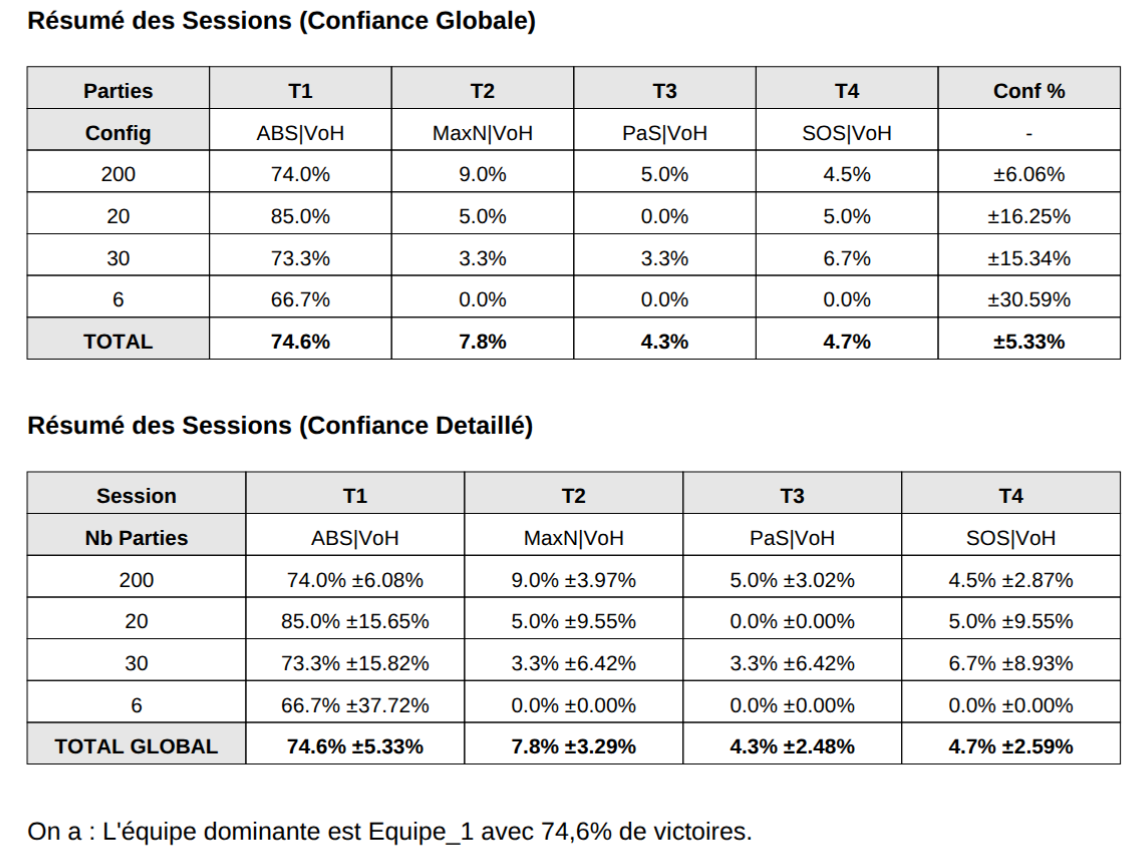
\includegraphics[width=0.9\linewidth]{images/analyse.png}
        \captionof{figure}{Impact de la profondeur de recherche.}
    \end{center}
\end{frame}

% ----- IMPACT DE LA PROFONDEUR -----
\begin{frame}{Impact de la profondeur de recherche}
    \begin{center}
        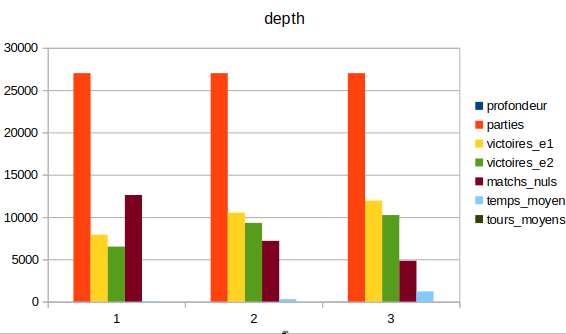
\includegraphics[width=0.9\linewidth]{images/depth.png}
        \captionof{figure}{Impact de la profondeur de recherche.}
    \end{center}
\end{frame}

% -----  COMPARAISON DES STRATÉGIES -----
\begin{frame}{Comparaison des stratégies}
    \begin{center}
        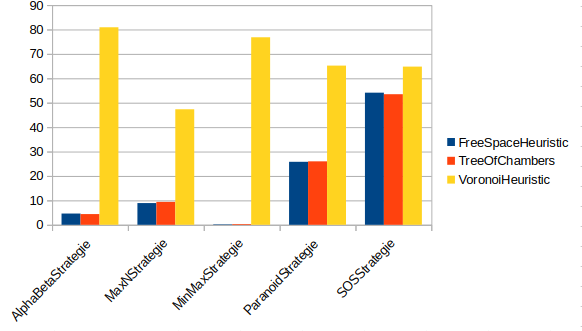
\includegraphics[width=1\linewidth]{images/coupleStratHeuristic.png}
        \captionof{figure}{Comparaison globale des stratégies avec les heuristiques}
    \end{center}
\end{frame}

% ==================== TESTS ====================
\begin{frame}{Tests principaux du projet}
    \begin{columns}[c]
        \begin{column}{0.32\textwidth}
            \begin{tcolorbox}[enhanced, arc=5pt, colback=softgreen, colframe=donecolor, title=\faCheckCircle Heuristiques]
                \centering
                \faCheckCircle~~VoronoiHeuristic\\
                \vspace{0.2cm}
                \faCheckCircle~~TreeOfChambersHeuristic\\
                \vspace{0.2cm}
                \faCheckCircle~~FreeSpaceHeuristic
            \end{tcolorbox}
        \end{column}
        \begin{column}{0.32\textwidth}
            \begin{tcolorbox}[enhanced, arc=5pt, colback=softblue, colframe=team2color, title=\faCheckCircle  Stratégies]
                \centering
                \faCheckCircle~~SOSStrategie\\
                \vspace{0.1cm}
                \faCheckCircle~~ParanoidStrategie\\
                \vspace{0.1cm}
                \faCheckCircle~~MinMaxStrategie\\
                \vspace{0.1cm}
                \faCheckCircle~~AlphaBetaStrategie
            \end{tcolorbox}
        \end{column}
        \begin{column}{0.32\textwidth}
            \begin{tcolorbox}[enhanced, arc=5pt, colback=softpurple, colframe=accentcolor, title=\faCheckCircle Modèle]
                \centering
                \faCheckCircle~~ModeleJeu
            \end{tcolorbox}
        \end{column}
    \end{columns}   
\end{frame}

% ==================== SLIDE 23 : OBJECTIFS ATTEINTS ====================
\section{Conclusion et perspectives}
\begin{frame}{Objectifs atteints et difficultés rencontrées}
    \begin{block}{Objectifs atteints}
        \begin{itemize}
            \item Implémentation de trois heuristiques : Voronoi, TreeOfChambers et FreeSpace.
            \item Développement de cinq stratégies : SOS, Paranoid, MinMax, AlphaBeta et MaxN.
            \item Mise en place du modèle, de l'interface graphique et des tests principaux.
            \item Ajout d'un mode d'expérimentation avec export CSV et PDF.
        \end{itemize}
    \end{block}

    \begin{alertblock}{Difficultés rencontrées}
        \begin{itemize}
            \item Certaines stratégies deviennent coûteuses quand la profondeur augmente.
            \item La complexité du jeu multi-joueurs rend les comparaisons difficiles.
            \item Le choix du protocole expérimental n'a pas été simple à cause des positions de départ aléatoires.
            \item Le multithreading améliore les performances, mais demande aussi plus de vigilance dans l'organisation des simulations.
        \end{itemize}
    \end{alertblock}
\end{frame}

% ==================== SLIDE 24 : PERSPECTIVES ====================
\begin{frame}{Perspectives d'amélioration}
    \begin{tcolorbox}[enhanced, arc=5pt, colback=softgreen, colframe=donecolor, title=Piste possible et validation future]
        \begin{itemize}
            \item Contrôle des positions de départ pour des comparaisons plus stables.
            \item Renforcement de l'analyse statistique des résultats.
            \item Extension du protocole expérimental à d'autres configurations.
            \item Optimisation des algorithmes de recherche.
        \end{itemize}
    \end{tcolorbox}
\end{frame}

% ==================== SLIDE 25 : BILAN ====================
\begin{frame}{Bilan du projet}
    \begin{tcolorbox}[enhanced, arc=5pt, colback=softblue, colframe=team1color, title=Points forts]
        \begin{itemize}
            \item Une architecture modulaire qui facilite l'ajout de nouvelles stratégies.
            \item Une diversité d'approches IA pour comparer plusieurs comportements.
            \item Un projet complet avec interface, expérimentation, export et tests.
        \end{itemize}
    \end{tcolorbox}

    \begin{tcolorbox}[enhanced, arc=5pt, colback=softgreen, colframe=donecolor, title=Apports du projet]
        \begin{itemize}
            \item Meilleure compréhension des algorithmes de recherche multi-agents.
            \item Travail en équipe avec le système de versioning Git.
            \item Première approche d'une analyse expérimentale sur un jeu compétitif.
        \end{itemize}
    \end{tcolorbox}

    \vspace{0.3cm}
    \begin{center}
        \textit{Ce projet nous a permis de relier conception logicielle, intelligence artificielle et expérimentation autour du jeu de Tron.}
    \end{center}
\end{frame}


% ==================== SLIDE 26 : FIN ====================
\begin{frame}[plain]
    \centering
    
    \begin{tikzpicture}[overlay, remember picture]
        \fill[team1color!10] (current page.south west) rectangle (current page.north east);
        \draw[team1color!30, line width=30pt] (current page.south west) -- (current page.north east);
    \end{tikzpicture}
    
    \vspace{1.5cm}
    
    {\Huge \color{team1color} \textbf{Merci pour votre attention !}}
    
    \vspace{0.5cm}
    
    \vspace{1cm}
    
    \begin{columns}[c]
        \begin{column}{0.45\textwidth}
            \centering
            \begin{tikzpicture}
                \node[circle, draw=team1color, thick, fill=team1color!20, inner sep=20pt, drop shadow, text=team1color] (q) {
                    \Huge \faQuestionCircle
                };
                \node[below=0.5cm of q, font=\large\bfseries, text=team1color] {Questions ?};
            \end{tikzpicture}
        \end{column}
        \begin{column}{0.45\textwidth}
            \centering
            \begin{tikzpicture}
                \node[circle, draw=accentcolor, thick, fill=accentcolor!20, inner sep=20pt, drop shadow, text=accentcolor] (s) {
                    \Huge \faLightbulb
                };
                \node[below=0.5cm of s, font=\large\bfseries, text=accentcolor] {Suggestions !};
            \end{tikzpicture}
        \end{column}
    \end{columns}
    
\end{frame}

\end{document}